
%\paragraph*{\color{purple}Context}
Most modern software systems can be customized via configuration options to meet user demands. Configuration options can enable desired functionality or tweak non-functional aspects of a software system, such as improving performance or energy consumption. The relationship of configuration choices and their influence on performance has been extensively studied in the literature~\cite{dorn2020,siegmundPerformanceinfluenceModelsHighly2015,haDeepPerf2019,perfAL,guoVariabilityawarePerformancePrediction2013,sarkarCostEfficientSamplingPerformance,guo_2018_data,fourier_learning_2015,perLasso}. The backbone of performance estimation are prediction models that map a given configuration to the estimated performance value. Learning performance models relies on a training set of configuration-specific performance measurements. In state-of-the-art approaches observations usually employ only a single workload which aims at emulating a specific real-world application scenario.

The choice of the workload (i.e., the input fed to the software system) is known to influence the performance of configurable software systems in different ways as has been shown for the domains of SAT solvers~\cite{falkner_sat_solvers_2015,satzilla_2008}, compilation~\cite{ding_compilation_2015,plotnikov_compilation_2013}, video transcoding~\cite{maxiaguine_workload_2004,alves_sampling_2020}, data compression~\cite{khavari_compression_2019}, and code verification~\cite{koc_satune_2021}. Besides apparent interactions, such as performance scaling with the size of a workload, qualitative aspects can result in more complex and non-trivial performance interactions.
{\color{novelblue}
Take as an example the distributions of configuration-specific throughput of the database \htwo in Figure~\ref{fig:h2_intro}. Here, we tested the exact same configurations on two different parameterizations of the benchmark TPC-C. The scale factor controlled the complexity (number of entities modeled) of the benchmark. While for most configurations, throughput decreases for a more complex benchmark, some configurations achieve higher throughput for a more complex benchmark. A similar example was outlined by~Pereira et al. for the video encoder \xzwo. That is, configuration-specific performance can be highly sensitive to workload variation and the behavior under different workloads can change in unforeseeable ways. In turn, this can render performance models based on a single workload useless, unless configuration options’ sensitivity to workloads is accounted for.
}
\begin{figure}
	\centering
	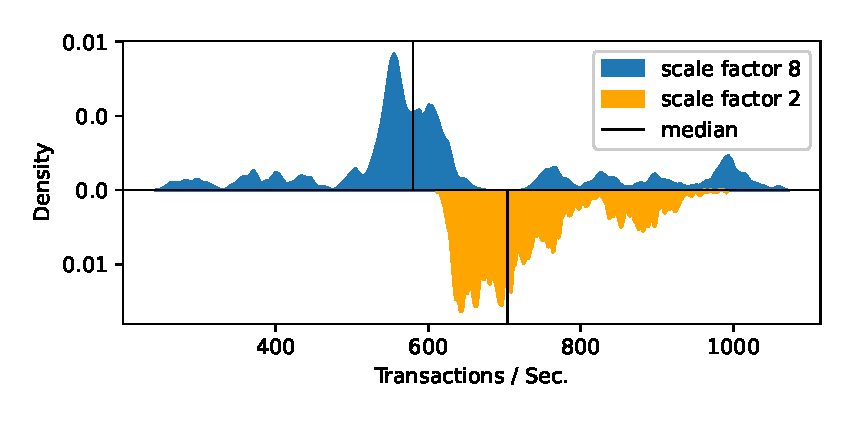
\includegraphics[width=0.95\linewidth]{images/h2_motivation.eps}
	\caption{Performance distributions of the database system \htwo run the \textsf{TPC-C} benchmark at different scale factors.}
	\label{fig:h2_intro}
\end{figure}

%\paragraph*{\color{purple}Motivation}
% ~\cite{jamishidi_transfer_2017,jamshidi_learning_2018,jamshidi_transfer_gp_2017}
To address this limitation, two different directions have been pursued in the literature. First, performance models trained using a specific workload can be adapted to another specific workload. Second,  one can specify workload characteristics as further independent variables when modeling configuration-dependent performance~\cite{koc_satune_2021}.
The first strategy direction relies on transfer learning techniques, where, given an existing performance model, in a separate step only the differences to a new environment are learned. Such a transfer function encodes which configuration options’ influence on performance is sensitive to workload variation. While transfer learning is an effective strategy that is not limited to varying workloads~\cite{jamshidi_learning_2018}, but can also be applied to different versions~\cite{jamishidi_transfer_2017,jamshidi_transfer_gp_2017,martin_transfer_2021}, or hardware setups~\cite{ding_bayesian_2020}, its main limitation is that the transfer function is specific to the differences between two environments.



In contrast to transfer learning, a more generalist approach is to consider the input fed to a software system as a further dimension for modeling performance. Here, a workload can be characterized by properties that---individually or in conjunction with software configuration options---influence performance. For such a strategy to work, one requires knowledge of the characteristics of a workload that influence performance. This strategy has been effectively tested for a  variety of application-domains, such as program verification. However, the added complexity comes at significant cost. 
Not only does this require substantially more measurements, we often lack knowledge of which performance-relevant characteristics best describe workloads.


%\paragraph*{\color{purple}Problem}
% ~\cite{khavari_compression_2019,maxiaguine_workload_2004,plotnikov_compilation_2013,ding_compilation_2015,falkner_sat_solvers_2015,satzilla_2008,alves_sampling_2020}
The existing body of research reflects the prevalence and importance of the workload influence on software systems. All these works are aware of the workload dimension as a factor of performance variation, yet little is known about the quality and driving factors of the \emph{interplay} between configuration options and workloads. Our understanding of this cross-factor relationship lacks knowledge of the following aspects:

\begin{compactitem}
	\item How different is configuration-specific performance across different workloads? 
	\item How many configuration options are responsible for differences in workload-specific performance behavior?
	\item What are the driving factors of the interplay between configuration options and workloads with regard to performance? 
\end{compactitem}

To answer these questions, we have conducted a systematic empirical study that sheds light on whether and how configuration options and workload choices interact with regard to performance. 
Specifically, {\color{red}we analyze 35\,659 configurations and 103 workloads across ten} configurable software systems to obtain a broad picture of the interaction of configuration and workload when learning performance models and estimating a configuration's performance (i.e., response time). Aside from studying the sole effects of workload variation on performance behavior, we explore possible driving factors. To this end, we enrich performance observations with corresponding statement coverage data to understand workload variation at finer granularity.

Our findings show that varying the workload can influence con\-fi\-gu\-ra\-tion-de\-pen\-dent software performance in different ways, including non-linear and non-monotonous effects. Our findings suggest that (a) coverage of code  specific to configuration options as well as (b) how such code is utilized are driving factors of input sensitivity. A key insight is that, to maintain and improve performance model representativeness, an additional notion of input sensitivity has to be considered. We argue that the use of code analysis techniques to address input sensitivity when varying the workload and maintain and improve the representativeness of a performance-prediction model.

To summarize, we make the following contributions: 

\begin{compactitem}
	\item {\color{red}An empirical study of 35\,659 configurations and 103 workloads across ten configurable software systems on whether interactions of workloads with configuration options affect performance and what factors can drive such interactions;}
	
	\item A detailed analysis that illustrates that variation in code coverage and code utilization due to varying workloads can affect the influence of configuration options on software performance; 
	
	\item A companion Web site\footnote{\url{https://github.com/fse-submission-2022/workload-performance/}} with supplementary material including performance and coverage measurements, experiment workloads and configurations, and an interactive dashboard\footnote{\url{https://workload-performance.herokuapp.com/}} for additional visualizations left out due to space limitations.
\end{compactitem}


